\documentclass[twoside]{article}

\usepackage[preprint]{aistats2027}
\usepackage{amsmath}
\usepackage{booktabs}
\usepackage{graphicx}
\usepackage{url}
\usepackage{fancyvrb}
\usepackage{xcolor}
\usepackage[square,numbers]{natbib}
\bibliographystyle{abbrvnat}
\usepackage{amsfonts}

\graphicspath{{figures/}}

\begin{document}

\runningtitle{Jev thinks ``I don't know'', but does not say it}
\runningauthor{Riccardo Porcedda}

\twocolumn[

\aistatstitle{Jev thinks ``I don't know'', but does not say it:\\Introducing Sys1Cal-v1 Dataset for Probability Calibration}

\aistatsauthor{Riccardo Porcedda}

\aistatsaddress{little-g.ai \\ Department of Excellence L'EMbeDS, Sant'Anna School of Advanced Studies, Italy \\ Department of Computer Science, University of Pisa, Italy} ]

\begin{abstract}
The appearance of Jev marked the era of System One Models, foundation models that return structured decisions with probability distributions rather than text. Aside from low cost and great speed, Jev's central promise is that these probabilities are calibrated: such claim is not backed by any public test and available external benchmarks evaluate confidence calibration, not whether every returned option probability has the right numerical meaning.
To tackle this issue, we introduce \textbf{Sys1Cal-v1}, a dataset of True/False questions about a proposition $A$ for which the exact probability $P(A)$ is known by construction. Each item is queried through the three Jev primitives - \texttt{Noul}, \texttt{Choice}, and \texttt{Score} - and evaluated by total variation distance from the ground-truth distribution, which can be used to estimate a soft accuracy of System One Models. We showcase the utility of Sys1Cal-v1 as a benchmark dataset by evaluating Jev and SemIf, an open-source \texttt{Choice}-style baseline. In particular, by studying the calibration of \texttt{Score} and \texttt{Choice} answers by Jev, we discover a peculiar behaviour that can be explained by assuming that Jev not only reasons in terms of True and False, but is capable of encoding a third truth value which is suppressed by default. In other words, in \texttt{Choice} answers $P(A)$ and $P(\neg A)$ are presented as if $P(A)+P(\neg A)=1$, while a term $P(U)\neq0$ is missing in the sum. Recovering $P(U)$ leads to an improvement of mean soft accuracy in \texttt{Choice} answers from $0.764$ to $0.931$, suggesting that, even in binary decisions, Jev wants to answer with a third option: \textit{``I don't know''}.
\end{abstract}

\section{Introduction}

Probabilistic predictions are often consumed by downstream decision rules rather than used only to select the most likely class. Under Bayesian decision theory, a predictive distribution is combined with task-dependent costs or utilities to determine an optimal action; consequently, reliable class probabilities are important for cost-sensitive classification, autonomous decision systems, and settings in which a model may abstain or defer uncertain cases \cite{gneiting2007proper,silvafilho2023classifier,chow1970optimum,elyaniv2010foundations}. This motivates predictive interfaces in which probabilities are first-class outputs rather than auxiliary confidence scores. Jev was introduced by TypeSafe AI as a \emph{System One Model} for this setting: given an input state and typed questions, it returns structured probabilistic decisions rather than free-form text, through \emph{\texttt{Noul}} for binary judgments, \emph{\texttt{Choice}} for categorical decisions, and \emph{\texttt{Score}} for ordered scales \cite{typesafe2026jev}.

Leaving aside the great speed and low cost of this model, a question arises about probability calibration, since no test on available public datasets was performed.
The importance of assessing this calibration for process automatization is decision-theoretic: for actions $a$, outcomes $y$, and utilities $u(a,y)$, the optimal downstream action depends on the predictive distribution,
\[
  a^*(x)=\arg\max_a \sum_y P(y\mid x)u(a,y).
\]
Argmax accuracy evaluates only the case of a binary decision, for which the probability distribution collapses to a label and discards precisely the information that downstream decisions may need.
To give some examples:
\begin{itemize}
    \item classical probabilistic calibration asks whether events assigned probability $p$ occur with frequency $p$ \cite{dawid1982wellcalibrated};
    \item proper scoring rules such as the Brier and logarithmic scores reward truthful predictive distributions in expectation \cite{brier1950verification,gneiting2007proper};
    \item recent work motivates posterior-probability evaluation from Bayes decision theory \cite{ferrer2024posterior};
    \item modern neural-network work popularized confidence calibration and expected calibration error (ECE), where only the probability of the predicted class is evaluated \cite{guo2017calibration}. The JevBench dataset \cite{jevbench_github} belongs to this category.
\end{itemize}
% For multiclass systems, however, confidence calibration, top-label calibration, classwise calibration, and full multiclass calibration are distinct properties \cite{vaicenavicius2019evaluating,kull2019dirichlet,gupta2021toplabel}. Moreover, empirical ECE depends on binning, class conditioning, norms, and estimator choices \cite{nixon2019measuring,kumar2019verified}. Classification accuracy is even coarser: it evaluates a single class decision and disregards probabilistic uncertainty information \cite{resin2023accuracy}.

% Existing JevBench-style evaluations are therefore incomplete for a typed probabilistic interface. JevBench reports accuracy, validity, latency, cost, Brier score, and top-label ECE over typed decisions \cite{jevbench_github}. Its public documentation states that ECE is computed from top-label confidence with 10 equal-width bins \cite{jevbench_github}. This is useful for measuring whether selected labels are overconfident,
Even if confidence calibration is an important test for System One models (we don't want class predictions to be underconfident/overconfident), this metric does not test whether each returned option probability has the right numerical meaning, whether equivalent states produce equivalent probabilities, or whether different Jev primitives expose compatible semantics (do probabilities from \texttt{Noul}, \texttt{Choice} and \texttt{Score} answers have the same meanings?).

We introduce \textbf{Sys1Cal-v1} to isolate that missing question. Sys1Cal-v1 is a synthetic dataset in which the exact probability of a proposition is known by construction, evaluating the model's probability distribution rather than only empirical calibration against one realized label.

\subsection{Contributions}

We make four contributions.

\textbf{First}, we introduce \textbf{Sys1Cal-v1}, a benchmark dataset of True/False questions about a proposition $A$ for which $P(A)$ is known.

\textbf{Second}, we show how Sys1Cal-v1 can be used to evaluate System One models. We report \textit{Distributional Overlap} (OVL), i.e., soft accuracy, for Jev across \texttt{Noul}, \texttt{Choice}, and \texttt{Score}, and for SemIf \cite{semif_repo} as a \texttt{Choice}-style open-source baseline.

\textbf{Third}, we identify a systematic \texttt{Choice} miscalibration in Jev. While the same problem is present also in SemIf, in Jev there is a mapping that appears to solve the problem, suggesting that there exist an underlying hidden process defining how Jev assigns probabilities.

\textbf{Finally}, we show that this hidden process can be the presence of a third truth value, the ambiguity $U$, which goes beyond the concepts of True and False and identifies a state of uncertainty of the model. Estimating $U$ and using it to fix the probability distribution of \texttt{Choice} answers, increases the mean soft accuracy from 0.764 to 0.931.



\section{Sys1Cal-v1}

\subsection{Dataset Design}

Each Sys1Cal-v1 item begins with the definition of a proposition $A$. A random generator produces the probability
\[
  p^* = P(A), \text{ therefore } P(\neg A)=1-p^*.
\]
From these, we generate the states, which in Sys1Cal-v1 are of six types: explicit probabilities, frequencies from counts, compound probability, conditional probability, Bayes' rule, and sequential Bayesian updates. 
The aim behind these six types is checking to what difficulty level a System One model is able to perform calibrated decisions.
Furthermore, the same problem can be rendered in multiple equivalent forms: direct probability statements, counts, ratios, tables, prose, nested state, and distractor-augmented state. 

In total, the first version of Sys1Cal-v1 contains 365 rendered examples derived from 92 problems.
Here is a simplified example of how a Sys1Cal-v1 item would look like:
\small
\begin{verbatim}
{
  "family": "explicit_probability",
  "representation": "direct",
  "state": {
    "sufficient_statistics": {
      "p_A": 0.105263157895,
      "p_not_A": 0.894736842105
    }
  },
  "queries": {
    "noul": {
      "proposition": "Event A is true."
    },
    "choice": {
      "question": "What is the truth status of the 
      following proposition?",
      "proposition": "Event A is true.",
      "options": ["False", "True"]
    },
    "score": {
      "question": "To what degree is the 
      following proposition true?",
      "proposition": "Event A is true.",
      "levels": [
        "Completely false",
        "Very strongly false",
        "Strongly false",
        "Moderately false",
        "Slightly false",
        "Slightly true",
        "Moderately true",
        "Strongly true",
        "Very strongly true",
        "Completely true"
      ]
    }
  }}
\end{verbatim}

\normalsize
% The actual dataset contains richer metadata and stable identifiers.

\begin{figure}[t]
\centerline{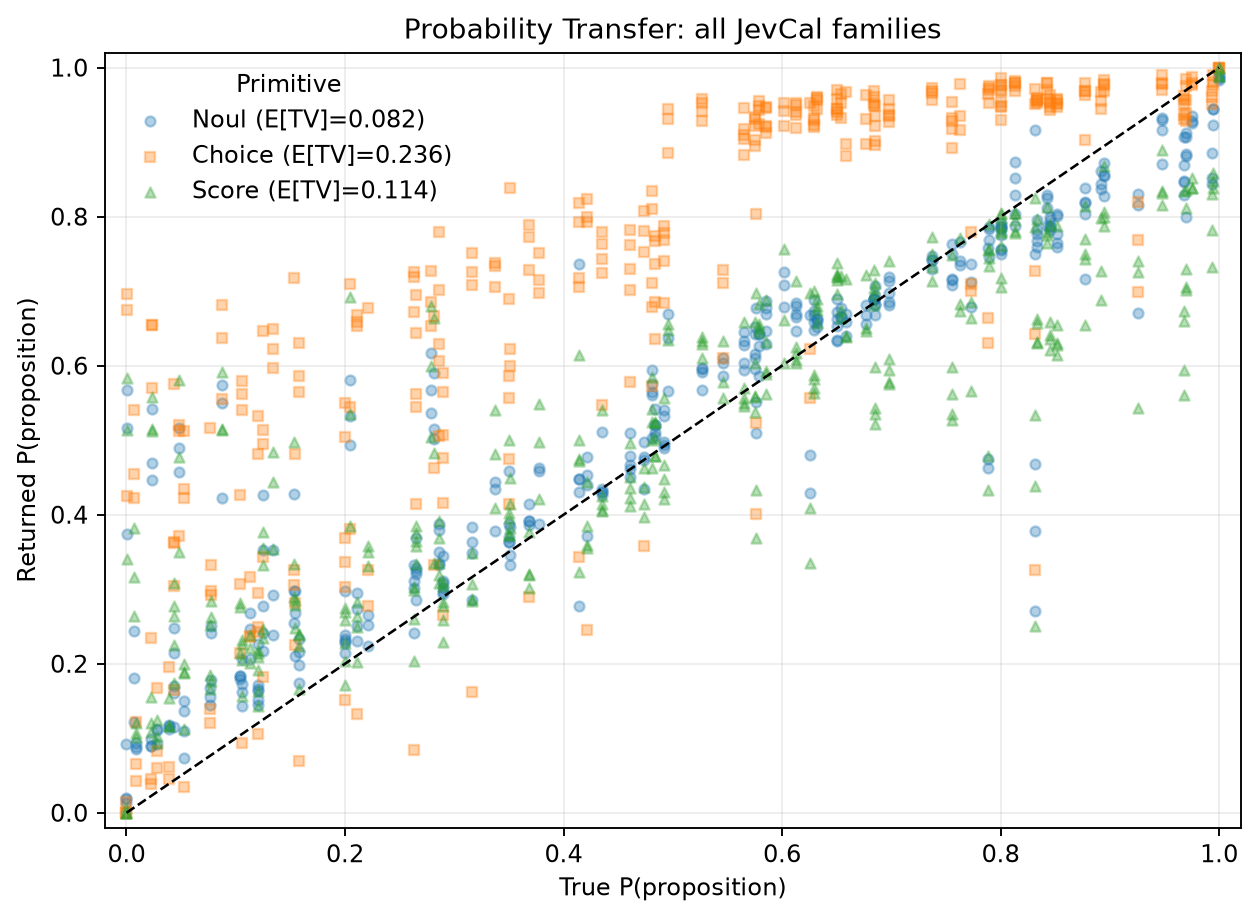
\includegraphics[width=\columnwidth]{figure_1_probability_transfer.png}}
\caption{Probability transfer across all Sys1Cal-v1 families. \texttt{Noul} and \texttt{Score} expectation remain closer to the dashed identity line, while \texttt{Choice} is systematically shifted toward high \texttt{True} probabilities.}
\label{fig:prob-transfer}
\end{figure}

\subsection{Primitives and Projections}
We are going to discuss now what we expect from Jev's primitives and how answers and their probabilities are evaluated through Sys1Cal-v1.

\paragraph{Noul}
The type \texttt{Noul} is the simplest primitive: if $A$ is the prompt, it returns the estimated probabilities $P(A)$ and $P(\neg A)$, with $P(A)+P(\neg A)=1$.
% We denote it by $p_N$.

\paragraph{Choice} This type returns a categorical distribution over defined criteria, i.e., possible answers to a given question. In our setting, the question is "What is the truth value of $A$?" and the criteria are \texttt{True} and \texttt{False}, therefore, we would expect the model to return $P(\texttt{True})=P(A)$ and $P(\texttt{False})=P(\neg A)$.
% We denote the probability assigned to \texttt{True} by $p_C$.

\paragraph{Score} This type returns an ordinal distribution over ordered, descriptive levels. So, for our purposes, while the question is the same as for \texttt{Choice}, here we define 10 levels corresponding to different grades of truth, from \texttt{Completely False} to \texttt{Completely True}. To each level $j$, we assign a numerical values $z_j=j/9$. The idea is to evaluate if the model is able to make fuzzy decisions.
Nonetheless, Sys1Cal-v1 only defines $P(\texttt{True})=P(A)$ and $P(\texttt{False})=P(\neg A)$, so, in order to evaluate probability calibration, we need a projection from numerical \texttt{Score} values into a binary \texttt{True}/\texttt{False} setting.

If $q_j$ is the score of level $j$ from the categorical distribution, and \texttt{Score} indeed represents a graded truth, we expect to get $P(A)$ from the \texttt{Score} \emph{expectation}
\begin{equation} \label{eq:score_exp}
    \mu_S=\sum_{j=0}^9 q_j z_j.
\end{equation}



\subsection{Metrics}

\begin{table}[t]
\caption{Mean TV and OVL (soft accuracy) by model-primitive. Jev-\texttt{Noul} and Jev-\texttt{Score} are well calibrated, while \texttt{Choice} answers show poorer performances on both Jev and SemIf}
\label{tab:main}
\begin{center}
% \setlength{\tabcolsep}{2.5pt}
% \scriptsize
\begin{tabular}{lrr}
\toprule
Output & Mean TV & Mean OVL \\
\midrule
Jev-\texttt{Choice} & 0.236 & 0.764 \\
Jev-\texttt{Noul} & 0.0817 & 0.918 \\
Jev-\texttt{Score} & 0.1139 & 0.886 \\
SemIf-\texttt{Choice} & 0.371 & 0.629 \\
\bottomrule
\end{tabular}
\end{center}
\end{table}

In Section \ref{sec:intro} we reported the main definitions of calibration. Here we set the metric used for System One models evaluation through Sys1Cal-v1: total variation distance.
Total variation distance is a statistical distance between two probability distributions (in this case, the true one and the empirical one returned ny the model). For a random variable that can take only two values, this is
\[
  \mathrm{TV}(\hat p,p^*) = |\hat p-p^*|,
\]
with $\hat p$ being the estimated probability and $p^*$ the real one.
From this, we can also define the \emph{Distributional Overlap} (OVL), also known as the overlapping coefficient \cite{inman1989overlap}:
\[
  \mathrm{OVL}(\hat p,p^*)=1-|\hat p-p^*|.
\]
This quantity lies in $[0,1]$ and can be considered a \emph{soft accuracy}, since it generalizes the accuracy metric from deterministic one-hot targets to probabilistic targets. Such a metric couldn't be adopted in benchmarks where only true labels are known, discarding their probability.
But Sys1Cal-v1 is constructed specifically to make the target distribution available for this type of evaluation.

We also adopt $\mathrm{TV}(\hat p,p^*)$ to measure representation sensitivity: while a proposition can be expressed in multiple ways, the values of $P(A)$ remain the same, so we would expect from a good System One model to return the same probabilities, regardless of the proposition being presented as prose, table, counts, or a ratio.
We therefore group problems in Sys1Cal-v1 and measure the pairwise TV distance between equivalent renderings of the proposition.
The full summary appears in Appendix~\ref{app:repr}.



\begin{figure*}[t]
\centerline{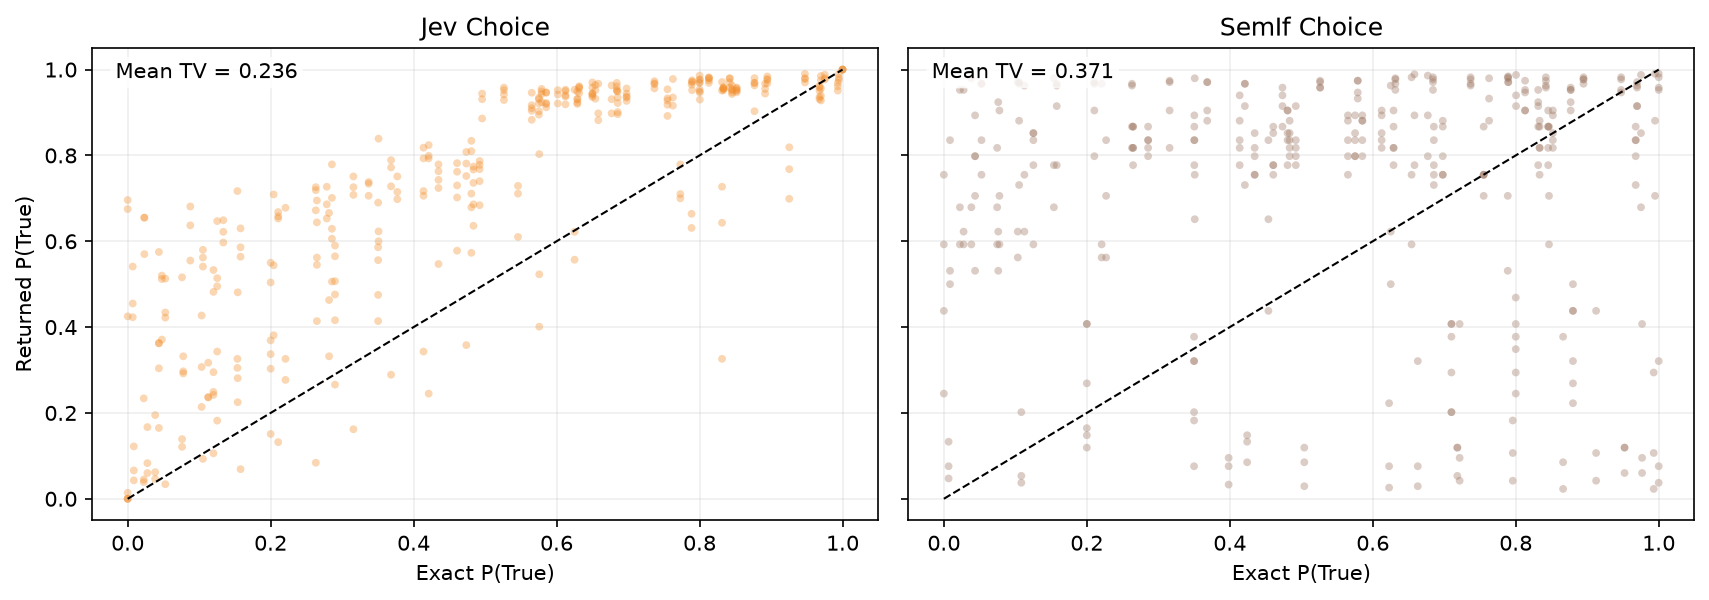
\includegraphics[width=\textwidth]{figure_26_choice_calibration_jev_semif.png}}
\caption{\texttt{Choice} probability transfer for Jev and SemIf. Mean TV is reported in each panel.}
\label{fig:choice-calibration}
\end{figure*}


\section{Evaluation of Probability Calibration}

Having defined the evluation metrics, we proceed with the experiments on probability calibration using Sys1Cal-v1.
Since Jev and SemIf outputs are not deterministic, we input each Sys1Cal-v1 item 10 times and obtain the corresponding answers' probabilities $p_1,...,p_{10}$, from which we estimate $\hat p=\sum_{i=1}^{10} p_i$. After this, we are able to compute $\mathrm{TV}(\hat p,p^*)$.

\subsection{Evaluating Primitives}
Instead of evaluating the overall probability calibration of the models, we want to study \texttt{Noul}, \texttt{Choice} and \texttt{Score} calibration separately. This is for two main reasons: having a fair comparison between Jev and SemIf (since the latter only produces \texttt{Choice} type answers) and studying in details the differences between Jev's primitives.
In Table~\ref{tab:main} we report the result.

While SemIf appears weaker in general, with an average OVL of 0.629, also Jev's \texttt{Choice} answers show worse calibration than \texttt{Noul} and \texttt{Score}. In Figure \ref{fig:prob-transfer} we provide a visual cue of this difference between primitives.
This is an interesting result, since, as we already highlighted, all the primitives are being evaluated on the same items and should estimate the same probabilities. In particular, it appears that Jev-\texttt{Choice} tends to return very high probabilities when $P(A)\geq0.5$, while being \emph{fuzzier} when $P(A)<0.5$. SemIf, on the other hand, appears to be generally miscalibrated (see Figure \ref{fig:choice-calibration}.



% \begin{table}[t]
% \caption{Cross-primitive semantic distances for Jev.}
% \label{tab:primitive}
% \begin{center}
% \footnotesize
% \begin{tabular}{@{}lrr@{}}
% \toprule
% Comparison & Mean abs. diff. & Median \\
% \midrule
% $|p_N - p_C|$ & 0.192 & 0.189 \\
% $|p_N - \mu_S|$ & 0.0541 & 0.0384 \\
% $|p_C - \mu_S|$ & 0.207 & 0.210 \\
% \midrule
% $p_C-p_N$ & 0.179 & 0.189 \\
% \bottomrule
% \end{tabular}
% \end{center}
% \end{table}





\begin{figure*}[t]
\centerline{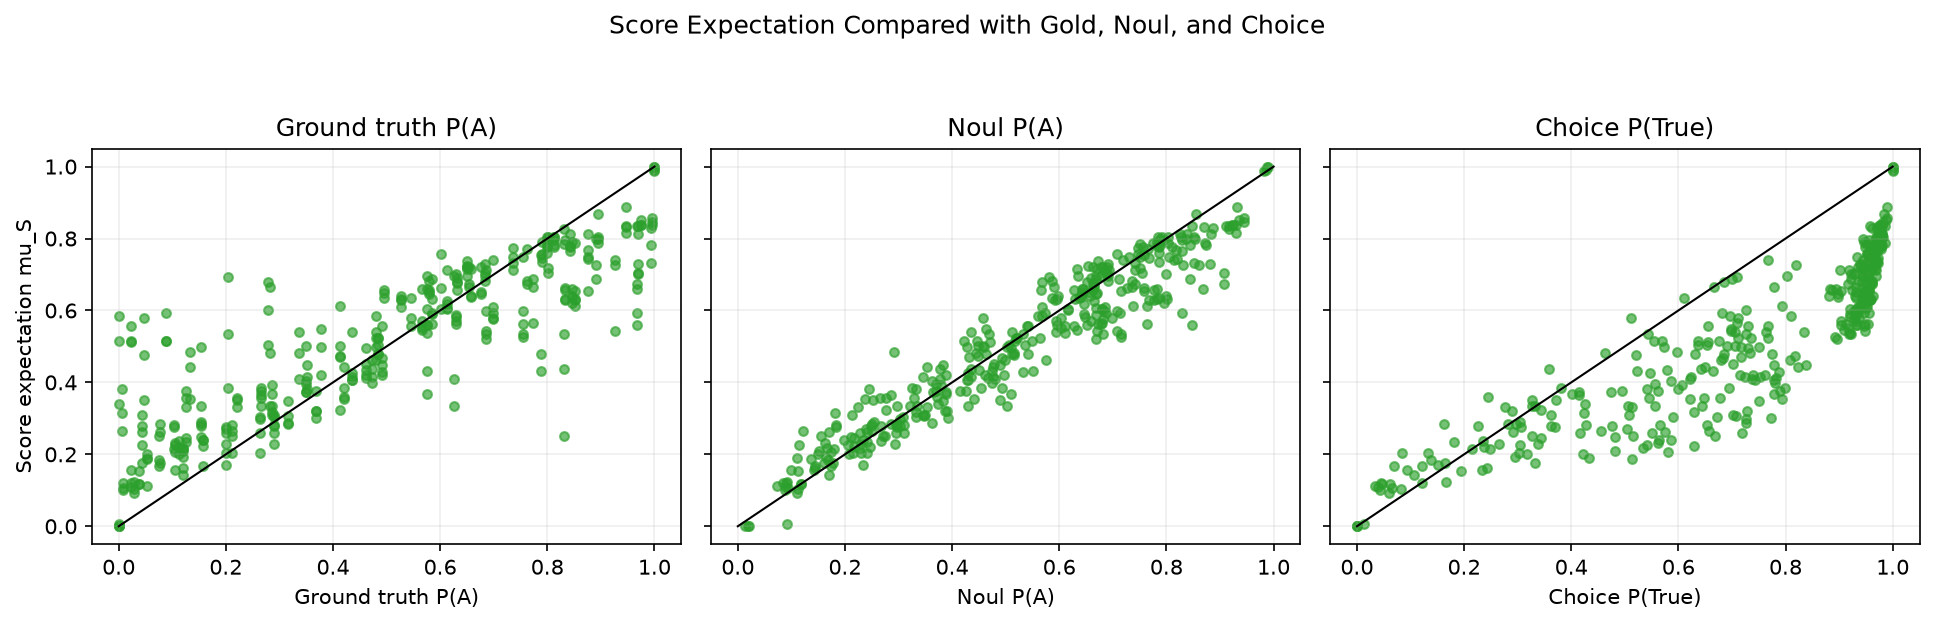
\includegraphics[width=\textwidth]{figure_8_score_expectation_connections.png}}
\caption{\texttt{Score} expectations compared with ground truth, \texttt{Noul}, and \texttt{Choice} probabilities. \texttt{Score} expectations tracks \texttt{Noul} more tightly than it tracks \texttt{Choice}, which shows a peculiar shape that suggests the existence of a map that could fix the calibration.}
\label{fig:score-connections}
\end{figure*}

Jev-\texttt{Noul} and Jev-\texttt{Score} show a similar calibration, obtaining an average OVL of $0.918$ and $0.886$, respectively, showing that the \texttt{Score} expectation defined in Equation \ref{eq:score_exp} correctly recovers the probabilities returned by Jev-\texttt{Noul}.
This also motivates us to furhter study the correlation between \texttt{Score} expectations and the probabilities returned by Jev-\texttt{Noul} and Jev-\texttt{Choice}.

\subsection{A hint from Score expectations}
In Figure \ref{fig:score-connections} we plot \texttt{Score} expectations against ground truth, \texttt{Noul}, and \texttt{Choice} probabilities. From the first plot, we can assess the goodness of the calibration of \texttt{Score} answers, and, in the second plot, we show the agreement between \texttt{Score} expectations and \texttt{Noul}.
But, more interestingly, the last plot shows that \texttt{Choice} answers are not merely miscalibrated: it appears that there exists a non-linear map from \texttt{Score} expectations that could fix the probability calibration.

This raises the following question: \textit{what kind of latent behavior would distort \texttt{Choice} probabilities in such a systematic way, while leaving \texttt{Noul} and \texttt{Score} expectation well correlated and much closer to the ground truth?}

% \section{Going Beyond True and False}

% \begin{figure}[t]
% \centerline{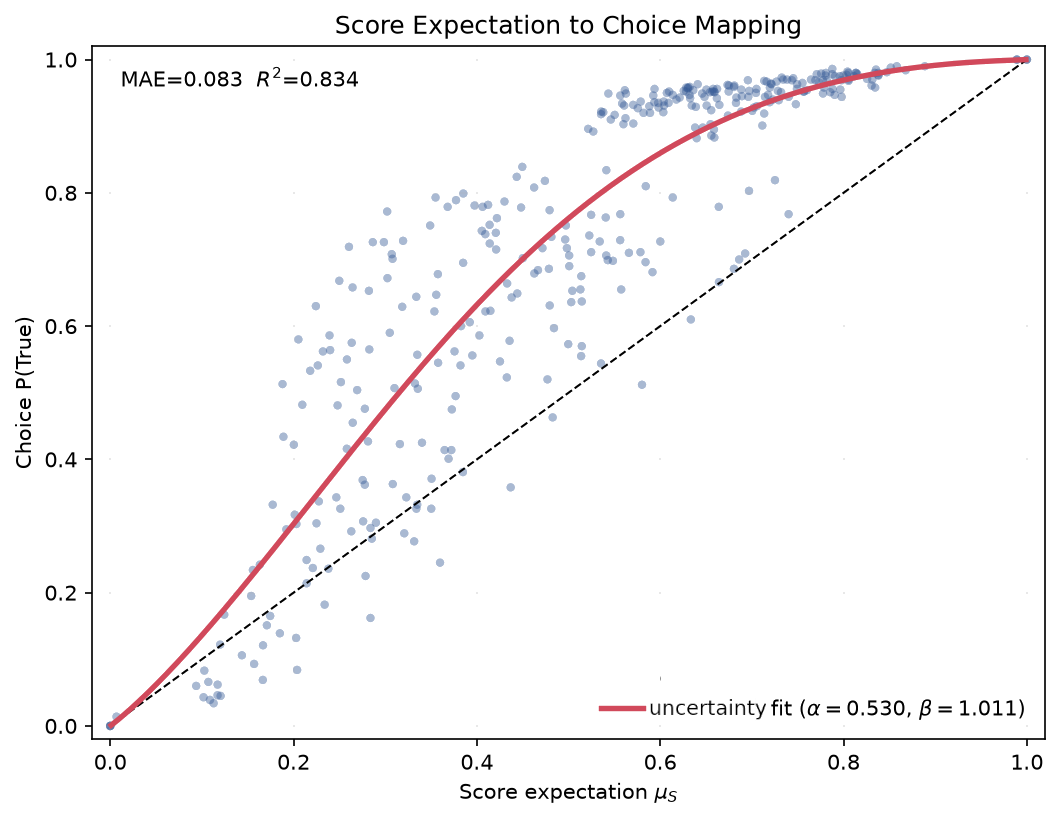
\includegraphics[width=\columnwidth]{figure_16_noul_choice_calibration.png}}
% \caption{\texttt{Score}-to-\texttt{Choice} mapping derived from two-exponent ambiguity mass. Ambiguity mass proportional to $\mu_S^\alpha(1-\mu_S)^\beta$ captures much of the systematic \texttt{Choice} distortion.}
% \label{fig:noul-choice}
% \end{figure}


% In Sys1Cal-v1, \texttt{Score} answers return an ordinal distribution from \texttt{Completely False} to \texttt{Completely True}, therefore allowing for multiple truth values that we later project into \texttt{True} and \texttt{False} with \texttt{Score} expectations as defined in Equation \ref{eq:score_exp}.

% Nonetheless, while this projection linearly correlates with \texttt{Noul} probabilities, the relation with \texttt{Choice} is non-linear, suggesting that a binary projection is not enough.
% We hypothesize the presence in \texttt{Choice} answers of an undisclosed third option, i.e., a third truth value, that we call \texttt{Uncertain}.

% Let
% \[
%   P(\texttt{True})+P(\texttt{Uncertain})+P(\texttt{False})=1.
% \]
% A forced binary \texttt{Choice} that discards $P(\texttt{Uncertain})$ would return
% \begin{align}
%   P_{\texttt{Choice}}(\texttt{True}) &= \frac{P(\texttt{True})}{P(\texttt{True})+P(\texttt{False})}\\
%   &=\frac{P(\texttt{True})}{1-P(\texttt{Uncertain})}.
% \end{align}

% We try to estimate $P(\texttt{Uncertain})$ \texttt{Score} expectations $\mu_S$ by assuming that uncertainty requires simultaneous support for truth and residual non-truth. We model it as
% \begin{equation}
%   P_{\alpha,\beta}(\texttt{Uncertain}|\mu_S)=\mu_S^\alpha(1-\mu_S)^\beta,
% \end{equation}
% with $\beta\ge 1$, so that $P_{\alpha,\beta}(\texttt{Uncertain}|\mu_S)\le 1-\mu_S$.

% Fitting this model to the data, we obtain $\alpha=0.530$, $\beta=1.011$, and $R^2=0.834$.
% To further assess the result, we test two null hypotheses:
% \begin{itemize}
%     \item there is no uncertainty;
%     \item there is no improvement in the prediction of \texttt{Choice} probabilities from \texttt{Score} expectations when introducing uncertainty.
% \end{itemize}.

% \begin{table}[t]
% \caption{Latent-level tests for the \texttt{Score}-ambiguity model. CIs use a normal approximation over 92 latent-problem means.}
% \label{tab:ambiguity-tests}
% \begin{center}
% \scriptsize
% \begin{tabular}{@{}lrrr@{}}
% \toprule
% Quantity & Mean & 95\% CI & $t$ \\
% \midrule
% $U_{\alpha,\beta}(\mu_S)>0$ & 0.292 & [0.276, 0.307] & 37.49 \\
% Abs. error improvement $>0$ & 0.110 & [0.0854, 0.135] & 8.67 \\
% \bottomrule
% \end{tabular}
% \end{center}
% \end{table}

% In Table~\ref{tab:ambiguity-tests} we shows that both null hypotheses are rejected.

% While our definition of uncertainty need not to be an exact discovery of how Jev encodes truth values, these tests prove that Jev for sure goes beyond a True/False-only setting.

% \section{Uncertainty as a Useful Signal}

% The inferred uncertainty is not merely a post-hoc explanation of calibration error. It is pragmatically useful.
% In selective prediction, a system may abstain when uncertainty is high; this is a standard way to trade coverage for reliability \cite{xin2021art}. Related work on language models has also shown that models can contain usable information about whether they know an answer, even when direct answer accuracy is imperfect \cite{kadavath2022language}.

% We may also check in Sys1Cal-v1 how the OVL of \texttt{Choice} answers is improved when the uncertainty is taken into account. A distribution $(T,U,F)$ specifies an interval of compatible truth probabilities,
% \[
%   P(A)\in[T,T+U].
% \]
% We therefore define the interval OVL score
% \[
%   \mathrm{OVL}_{TUF}
%   =
%   1-d\bigl(p^*,[T,T+U]\bigr),
% \]
% where $d$ is absolute distance from the point $p^*$ to the interval. This reduces to ordinary binary OVL when $U=0$.
% In Sys1Cal-v1 \texttt{Choice} answers, $\mathrm{OVL}_{TUF}$ reaches 0.931, against $\mathrm{OVL}=0.764$ in the \texttt{True/False} setting (see Figure \ref{fig:selective-unknown}).

% \begin{figure}[t]
% \centerline{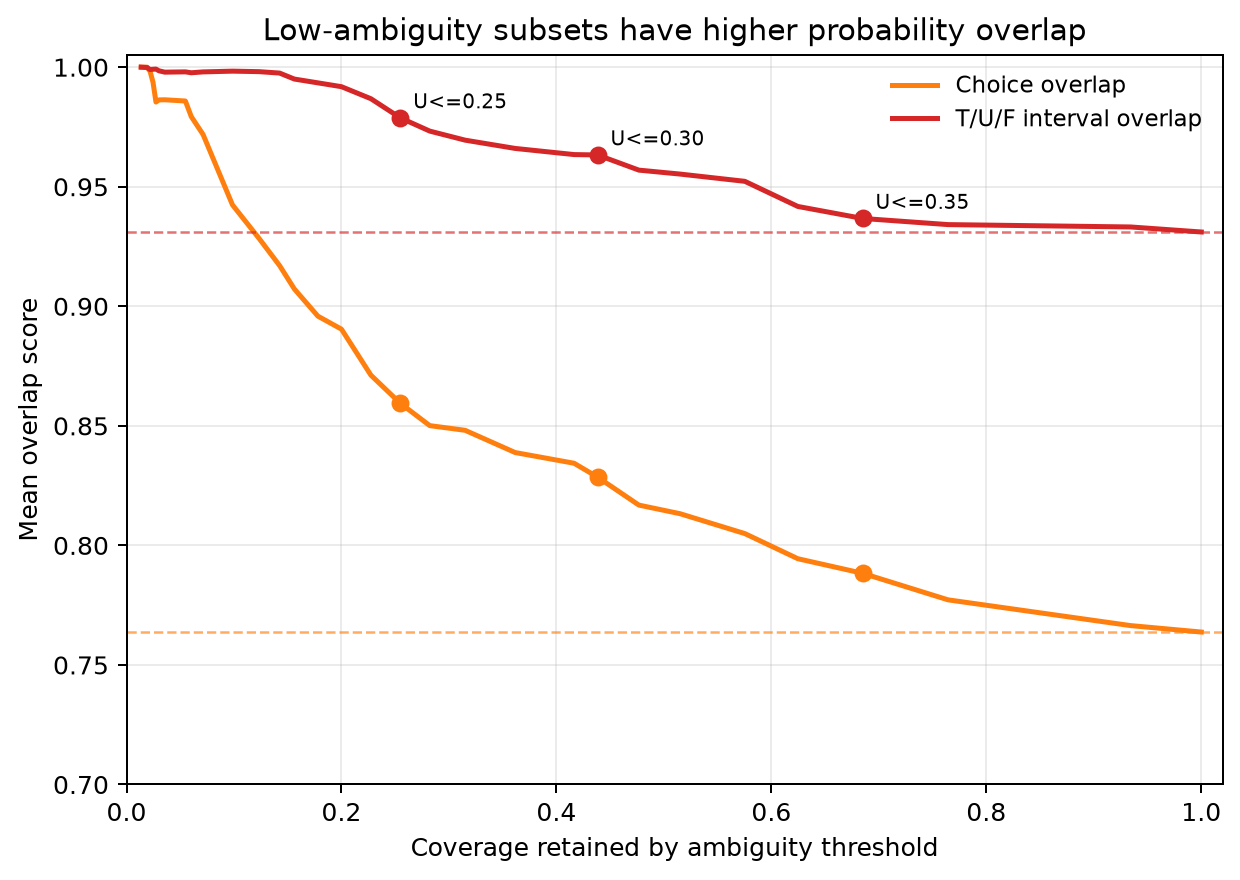
\includegraphics[width=\columnwidth]{figure_23_unknown_selective_accuracy.png}}
% \caption{Mean OVL after retaining items with low ambiguity mass. Dashed lines show full-coverage means. Low ambiguity corresponds to better \texttt{Choice} probability overlap, while the inferred $(T,U,F)$ interval remains highly compatible with the gold probability.}
% \label{fig:selective-unknown}
% \end{figure}


% \paragraph{Decision-theoretic interpretation.}
% Here we give an example of how Jev uncertainty, if not disclosed, can lead to non-ideal decisions.
% Let $P_{\texttt{Choice}}(\texttt{A is True})=0.8$ and $P_{\texttt{Choice}}(\texttt{A is False})=0.2$.
% Consider a decision problem in which an agent can either act as if the proposition is true ($a_T$), act as if it is false ($a_F$), or defer the decision to another agent ($a_D$) to get the right answer. Assume that an incorrect committed decision has cost $C_{\mathrm{err}}=100$, while deferring has cost $C_D=30$. In the binary \texttt{Choice} setting, the expected losses are
% \[
% R(a_T)=100\,P(F)=20,\\
% R(a_F)=100\,P(T)=80,\\
% R(a_D)=30,
% \]
% so the Bayes-optimal action is to commit to $a_T$. In the latent \texttt{True}/\texttt{Uncertain}/\texttt{False} representation, instead, our uncertainty model gives
% \[
% P(\texttt{A is True})=0.535,\\
% P(\texttt{A is Uncertain})=0.331,\\
% P(\texttt{A is False})=0.134.
% \]
% This induces the credal interval
% \[
% P(T)\in[\underline p,\overline p]
% =[T,T+U]=[0.535,0.866].
% \]
% Under a robust $\Gamma$-minimax decision rule, each committed action is evaluated according to its largest expected loss over this set. Hence,
% \[
% \overline R(a_T)
% =100(1-\underline p)=46.5,
% \qquad
% \overline R(a_F)
% =100\,\overline p=86.6,
% \qquad
% \overline R(a_D)=30.
% \]
% The optimal decision therefore changes from \emph{commit to True} in the binary representation to \emph{defer} in the $T/U/F$ representation. Importantly, both representations still agree on the direction of the decision if commitment is forced: indeed,
% \[
% \frac{T}{T+F}
% =\frac{0.535}{0.535+0.134}
% \simeq 0.8.
% \]
% The difference is therefore not which alternative is preferred, but whether the available evidence is sufficient to justify committing to it given the cost of an error and the cost of acquiring further information.


% At full coverage, \texttt{Choice} OVL is 0.764. Keeping items with $U\le 0.30$ gives 43.8\% coverage and raises \texttt{Choice} OVL to 0.829; with $U\le 0.25$, coverage is 25.5\% and \texttt{Choice} OVL is 0.859. The corresponding interval OVL scores are 0.963 and 0.979. Thus ambiguity improves evaluation in a probability-native sense: it identifies examples where the binary \texttt{Choice} distribution is closer to the true probability, and it supplies a three-status interval that is highly compatible with $p^*$.

% This also clarifies why probability calibration matters for automation. A binary \texttt{Choice} probability can be wrong because the model may not simply be choosing between true and false; it may be compressing true, false, and unresolved mass into two reported options. When that unresolved mass is estimated from ambiguity, downstream systems can make better decisions about when to trust, defer, or request more evidence.


\section{Going Beyond True and False}

In Sys1Cal-v1, \texttt{Score} answers return an ordinal distribution
ranging from \texttt{Completely False} to \texttt{Completely True}.
We summarize this distribution through its expectation $\mu_S$, as
defined in Equation~\ref{eq:score_exp}. A direct binary interpretation
would therefore associate $\mu_S$ with the probability of
\texttt{True} and $1-\mu_S$ with the probability of \texttt{False}.

As we have shown, this projection is linearly related to
\texttt{Noul} probabilities. Its relation with binary
\texttt{Choice} probabilities, however, is non-linear.
This suggests that the transformation from \texttt{Score} to
\texttt{Choice} may discard information that cannot be represented by
a direct True/False projection.

We therefore introduce a latent three-component probability
distribution
\begin{equation*}
    \pi_T+\pi_U+\pi_F=1,
\end{equation*}
where $\pi_T$, $\pi_U$, and $\pi_F$ denote, respectively, the latent
probabilities associated with \texttt{True}, \texttt{Uncertain}, and
\texttt{False}.

If \texttt{Choice} excludes the uncertain component and renormalizes
the remaining two probabilities, then
\begin{align}
P_{\texttt{Choice}}(\texttt{True})
    &=
    \frac{\pi_T}{\pi_T+\pi_F}
    \\
    &=
    \frac{\pi_T}{1-\pi_U},
\label{eq:choice-renorm}
\end{align}
and analogously
\[
P_{\texttt{Choice}}(\texttt{False})
=
\frac{\pi_F}{1-\pi_U}.
\]

We infer this latent representation from the \texttt{Score}
expectation $\mu_S$. In particular, we take the \texttt{Score}
expectation as the latent probability already assigned to
\texttt{True},
\begin{equation}
    \widehat{\pi}_T=\mu_S,
\end{equation}
and allow part of the remaining probability $1-\mu_S$ to represent
uncertainty.
The reason why we assume this is that \texttt{Score}
expectations and \texttt{Choice} answers (which are strongly correlated) appear to be well calibrated, so no relevant uncertainty appears to be present in $\mu_S$.

We model this latent uncertainty probability as
\begin{equation*}
    \widehat{\pi}_U(\mu_S)
    =
    \mu_S^\alpha(1-\mu_S)^\beta,
\label{eq:latent-uncertainty}
\end{equation*}
with $\alpha>0$ and $\beta\geq1$. These constraints guarantee that
\[
0\leq \widehat{\pi}_U(\mu_S)\leq 1-\mu_S.
\]
The remaining probability is assigned to \texttt{False},
\begin{equation*}
    \widehat{\pi}_F
    =
    1-\widehat{\pi}_T-\widehat{\pi}_U.
\end{equation*}

The corresponding prediction of the binary \texttt{Choice}
probability is therefore
\begin{equation*}
\widehat{P}_{\texttt{Choice}}(\texttt{True}\mid\mu_S)
=
\frac{\mu_S}
{1-\mu_S^\alpha(1-\mu_S)^\beta}.
\label{eq:score-choice-model}
\end{equation*}

Fitting this model to Sys1Cal-v1 yields
\[
\alpha=0.530,
\qquad
\beta=1.011,
\]
with $R^2=0.834$ for the resulting prediction of
\texttt{Choice} probabilities (see Figure \ref{fig:noul-choice}).


More importantly, introducing this
component improves the prediction of binary \texttt{Choice}
probabilities: the mean reduction in absolute error is $0.110$, with
a 95\% confidence interval that excludes zero.

While our definition of uncertainty need not to be an exact discovery of how Jev encodes truth values, these tests show that \textbf{Jev-\texttt{Choice} may go beyond a True/False-only setting}.

\begin{figure}[t]
\centerline{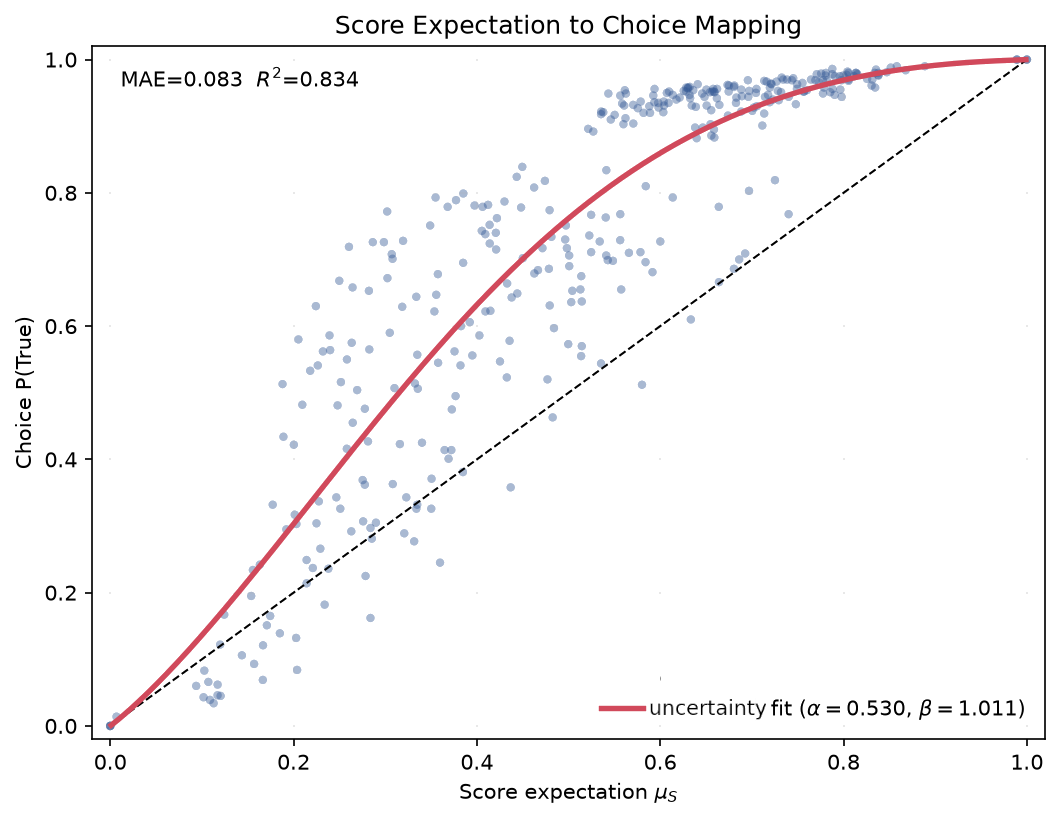
\includegraphics[width=\columnwidth]{figure_16_noul_choice_calibration.png}}
\caption{
\texttt{Score}-to-\texttt{Choice} mapping induced by the fitted latent
uncertainty model. Introducing a latent uncertainty probability of the
form $\mu_S^\alpha(1-\mu_S)^\beta$ captures much of the systematic
non-linearity between \texttt{Score} expectations and binary
\texttt{Choice} probabilities.
}
\label{fig:noul-choice}
\end{figure}

\section{Uncertainty as a Useful Signal}

The inferred uncertainty probability is not only useful for explaining
the transformation from \texttt{Score} to \texttt{Choice} and adjusting the calibration of the latter primitive. It also
contains information that can be exploited by downstream systems.

Consider a latent distribution
\[
(\pi_T,\pi_U,\pi_F).
\]
The components $\pi_T$ and $\pi_F$ represent probability already
committed to \texttt{True} and \texttt{False}, respectively, whereas
$\pi_U$ remains unresolved. If the uncertain component may ultimately
resolve toward either outcome, then the latent distribution does not
specify a unique binary truth probability. Instead, it induces the set
of compatible probabilities
\begin{equation}
p=P(\texttt{True})
\in
[\pi_T,\pi_T+\pi_U].
\label{eq:credal-interval}
\end{equation}
The lower bound corresponds to assigning all unresolved probability to
\texttt{False}, whereas the upper bound corresponds to assigning it
entirely to \texttt{True}.

Thus, the latent representation naturally defines a simple credal
interval over the binary proposition. Its width is exactly the latent
uncertainty probability,
\begin{equation*}
(\pi_T+\pi_U)-\pi_T=\pi_U.
\end{equation*}

This interpretation also suggests an interval-valued extension of the
OVL metric. Given the gold probability $p^*$, we define
\begin{equation*}
\mathrm{OVL}_{TUF}
=
1-
d\!\left(
p^*,
[\widehat{\pi}_T,
 \widehat{\pi}_T+\widehat{\pi}_U]
\right),
\label{eq:interval-ovl}
\end{equation*}
where $d(p,I)$ denotes the absolute distance between a point $p$ and
an interval $I$. In particular,
\[
d(p,[a,b])
=
\begin{cases}
a-p, & p<a,\\
0,   & a\leq p\leq b,\\
p-b, & p>b.
\end{cases}
\]
When $\widehat{\pi}_U=0$, the interval collapses to a single
probability and $\mathrm{OVL}_{TUF}$ reduces to ordinary binary OVL.

On Sys1Cal-v1, the latent interval representation reaches
\[
\mathrm{OVL}_{TUF}=0.931,
\]
compared with
\[
\mathrm{OVL}=0.764
\]
for the corresponding binary \texttt{Choice} probabilities.

\begin{table}[t]
  \caption{Tests for the scaled Score--Uncertainty model.
  The null hypothesis is $H_0:\lambda=0$.
  The global $\hat\lambda$ row reports the fitted scale and a bootstrap
  confidence interval over latent problems. The $\lambda_j$ tests whether the fitted uncertainty is positive across the latent problems.}
  \label{tab:ambiguity-tests}
  \begin{center}
  \begin{tabular}{lrrr}
  \toprule
  Quantity & Estimate & 95\% CI & $p$-value \\
  \midrule
  Global $\hat\lambda$ & 0.978 & [0.789, 1.000] & -- \\
  Latent $\lambda_j$ & 0.821 & [0.760, 0.882] & $2.94{\times}10^{-44}$ \\
  \bottomrule
  \end{tabular}
  \end{center}
\end{table}

\paragraph{Decision-theoretic interpretation.}

The uncertainty probability is also informative for selective
prediction. In selective prediction, a system may abstain or defer on
uncertain examples in order to trade coverage for reliability
\cite{xin2021art}. Related work on language models has similarly shown
that models may contain useful information about whether their answers
are reliable even when direct answer accuracy is imperfect
\cite{kadavath2022language}.

% \begin{figure}[t]
% \centerline{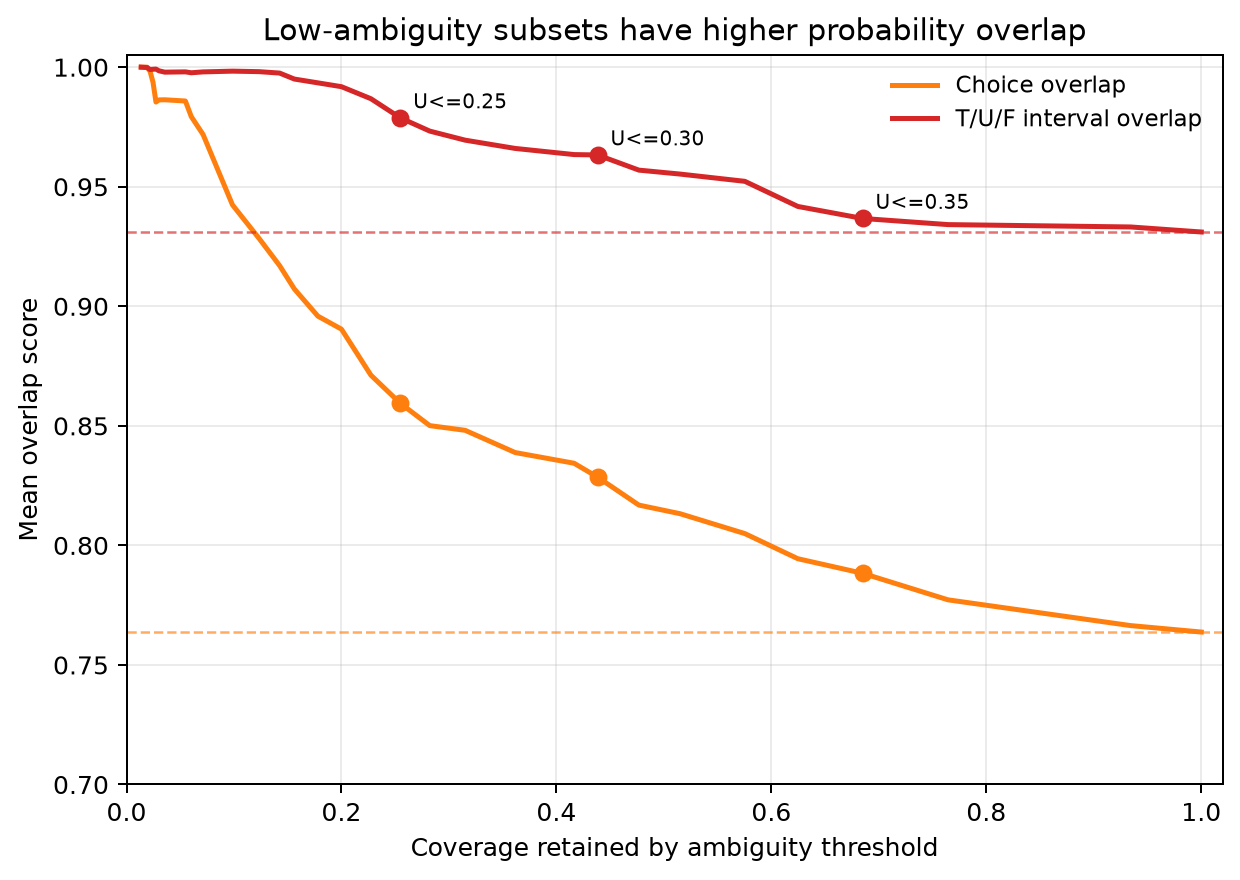
\includegraphics[width=\columnwidth]{figure_23_unknown_selective_accuracy.png}}
% \caption{
% Mean OVL after retaining examples with low inferred uncertainty
% probability $\widehat{\pi}_U$. Dashed lines indicate full-coverage
% performance. Lower uncertainty identifies examples for which the
% binary \texttt{Choice} probability is closer to the gold probability,
% while the corresponding latent probability interval remains highly
% compatible with it.
% }
% \label{fig:selective-unknown}
% \end{figure}

% At full coverage, binary \texttt{Choice} achieves an OVL of $0.764$.
% Restricting evaluation to examples with
% $\widehat{\pi}_U\leq0.30$ retains $43.8\%$ of the data and raises
% binary OVL to $0.829$. With
% $\widehat{\pi}_U\leq0.25$, coverage decreases to $25.5\%$, while
% binary OVL increases further to $0.859$. The corresponding interval
% OVL scores are $0.963$ and $0.979$, respectively.

% These results show that the inferred uncertainty probability is useful
% in two complementary ways. First, low $\widehat{\pi}_U$ identifies
% examples for which the forced binary \texttt{Choice} probability is
% more reliable. Second, when $\widehat{\pi}_U$ is large, the interval
% \[
% [\widehat{\pi}_T,
%  \widehat{\pi}_T+\widehat{\pi}_U]
% \]
% represents the range of binary truth probabilities compatible with the
% unresolved component.


% The distinction between the binary \texttt{Choice} probability and the
% latent representation becomes particularly relevant when

Let's consider a situation in which an agent faces a costly decision.

Let the true state be either \texttt{True} or \texttt{False}, and
consider three available actions:
\[
a_T=\text{act as if the proposition is True},
\]
\[
a_F=\text{act as if the proposition is False},
\]
\[
a_D=\text{defer the decision}.
\]
Assume that a correct committed decision has zero loss, an incorrect
committed decision has cost
\[
C_{\mathrm{err}}=100,
\]
and deferring the decision to a more reliable procedure has cost
\[
C_D=30.
\]
For simplicity, we assume that deferral resolves the uncertainty before
a final action is taken.

Suppose that the binary \texttt{Choice} output is
\[
P_{\texttt{Choice}}(\texttt{True})=0.8,
\qquad
P_{\texttt{Choice}}(\texttt{False})=0.2.
\]
Under standard Bayesian decision theory, the expected losses are
\begin{align*}
R(a_T)
    &=100\cdot P_{\texttt{Choice}}(\texttt{False})
      =20,\\
R(a_F)
    &=100\cdot P_{\texttt{Choice}}(\texttt{True})
      =80,\\
R(a_D)
    &=30.
\end{align*}
The Bayes-optimal action is therefore $a_T$.

Now consider the latent representation inferred from the same
\texttt{Score} answer,
\[
(\widehat{\pi}_T,
 \widehat{\pi}_U,
 \widehat{\pi}_F)
=
(0.535,0.331,0.134).
\]
After excluding the uncertainty probability and renormalizing the two
committed components, Equation~\ref{eq:choice-renorm} gives
\[
\frac{\widehat{\pi}_T}
     {\widehat{\pi}_T+\widehat{\pi}_F}
=
\frac{0.535}{0.535+0.134}
\simeq0.8.
\]
Thus, the binary and latent representations agree on the preferred
direction of the decision when commitment is mandatory.

However, the latent representation contains additional information.
From Equation~\ref{eq:credal-interval}, it induces the compatible
binary probability interval
\[
p=P(\texttt{True})
\in
[0.535,0.866].
\]

If the latent representation is interpreted as defining a set
$\Gamma$ of compatible binary probability distributions, a natural
robust decision criterion is the $\Gamma$-minimax rule
\cite{berger1985statistical,walley1991statistical},
\begin{equation*}
a^*
=
\arg\min_{a}
\sup_{P\in\Gamma}
\mathbb{E}_{P}[L(a,\theta)].
\end{equation*}

For $a_T$, the worst case
is the smallest compatible probability of \texttt{True}; for $a_F$,
it is the largest. Hence,
\begin{align*}
\overline{R}(a_T)
    &=
    100(1-0.535)
    =
    46.5,\\
\overline{R}(a_F)
    &=
    100(0.866)
    =
    86.6,\\
\overline{R}(a_D)
    &=
    30.
\end{align*}
The robust optimal action is therefore
$a_D$.

The two representations consequently lead to different optimal
decisions. Using only the binary \texttt{Choice} probability, the
agent commits to \texttt{True}. Once the inferred uncertainty
probability is retained, the agent instead defers.

Importantly, the disagreement is not about which outcome is preferred.
\textit{Both representations favor \texttt{True} if a binary commitment is
forced. The difference concerns whether commitment is justified given
the cost of making an error relative to the cost of obtaining further
information.}

% The binary \texttt{Choice} probability describes the
% relative preference between \texttt{True} and \texttt{False} after the
% uncertainty component has been excluded, whereas the latent
% representation additionally quantifies how much probability remains
% unresolved before that forced binary decision.


\section{Scope and Limitations}

Sys1Cal-v1 is designed to isolate probability semantics, not to measure broad natural-language competence. Its synthetic construction is a strength because it gives exact pointwise probabilities, but it also limits ecological coverage: future releases should include richer language variation, adversarial paraphrases, and domain-specific probability tasks. Our \texttt{Score} analysis uses the expectation of a 10-level distribution as a scalar truth-probability projection; other projections may expose additional structure. Finally, the uncertainty model is an observational explanation of the relation between \texttt{Score} and \texttt{Choice} outputs. It supports the hypothesis that \texttt{Choice} behaves like a binary collapse of a richer representation, but it is not a causal claim about Jev's internal architecture.



\section{Conclusion}

We introduced Sys1Cal-v1, a benchmark for evaluating whether the
probabilities returned by System One models have the intended numerical
meaning. Unlike standard calibration benchmarks, Sys1Cal-v1 provides the
exact probability of each proposition by construction and evaluates the
full predictive distribution rather than only confidence in the selected
label. This makes it possible to compare probabilistic semantics across
different primitives and across equivalent representations of the same
underlying problem.

Our evaluation shows that Jev's primitives do not expose probability in
the same way. \texttt{Noul} and \texttt{Score} are substantially better
aligned with the ground-truth probabilities than \texttt{Choice}. The same benchmark also reveals
representation sensitivity: equivalent formulations of the same
probability problem can induce different outputs, with \texttt{Choice}
being less invariant than \texttt{Noul} and \texttt{Score}.

We also show that \texttt{Choice} miscalibration can be explained by assuming a non-disclosed third truth value \texttt{Uncertain}.
The inferred uncertainty model reduces the miscalibration of \texttt{Choice}, increasing mean OVL, i.e., soft accuracy, from
$0.764$ for the reported binary \texttt{Choice} probabilities to
$0.931$.

The discovered presernce of a third truth value carries information that can be relevant to
downstream decision making, in particular to evluate when a decision should be deferred.

This distinction matters because probabilistic outputs are ultimately
used to choose actions. A forced binary probability may indicate which
action is preferred if a decision must be made, while the latent
uncertainty probability can determine whether committing to that action
is justified at all. When abstention, escalation, or information
acquisition are available, suppressing uncertainty can therefore change
the optimal decision.

Our results suggest that evaluating structured decision models requires going beyond
argmax accuracy and confidence calibration: if probabilities are meant to
support automated decisions, then their semantics---including the
probability that remains unresolved---must be appropriately evaluated.



% Bibliography
\bibliography{main}

% \begin{thebibliography}{99}

% \bibitem[JevBench Repository(2026)]{jevbench_github}
% JevBench Repository.
% \newblock \emph{JevBench v1: A benchmark for Jev-class typed decision models}.
% \newblock \url{https://github.com/fstandhartinger/jevbench}, accessed September 22, 2026.

% \bibitem[SemIf Repository(2026)]{semif_repo}
% SemIf Repository.
% \newblock \emph{SemIf: Open baselines for runtime-defined semantic decisions}.
% \newblock \url{https://github.com/TheoLeeCJ/SemIf}, accessed September 23, 2026.

% \bibitem[Dawid(1982)]{dawid1982wellcalibrated}
% A.~Philip Dawid.
% \newblock The well-calibrated Bayesian.
% \newblock \emph{Journal of the American Statistical Association}, 77(379):605--610, 1982.

% \bibitem[Brier(1950)]{brier1950verification}
% Glenn~W. Brier.
% \newblock Verification of forecasts expressed in terms of probability.
% \newblock \emph{Monthly Weather Review}, 78(1):1--3, 1950.

% \bibitem[Gneiting and Raftery(2007)]{gneiting2007proper}
% Tilmann Gneiting and Adrian~E. Raftery.
% \newblock Strictly proper scoring rules, prediction, and estimation.
% \newblock \emph{Journal of the American Statistical Association}, 102(477):359--378, 2007.

% \bibitem[Inman and Bradley(1989)]{inman1989overlap}
% Henry~F. Inman and Edwin~L. Bradley.
% \newblock The overlapping coefficient as a measure of agreement between probability distributions and point estimation of the overlap of two normal densities.
% \newblock \emph{Communications in Statistics -- Theory and Methods}, 18(10):3851--3874, 1989.

% \bibitem[Guo et~al.(2017)]{guo2017calibration}
% Chuan Guo, Geoff Pleiss, Yu Sun, and Kilian~Q. Weinberger.
% \newblock On calibration of modern neural networks.
% \newblock \emph{Proceedings of the International Conference on Machine Learning}, 2017.

% \bibitem[Kull et~al.(2019)]{kull2019dirichlet}
% Meelis Kull, Miquel Perello Nieto, Markus K{\"a}ngsepp, Telmo Silva Filho, Hao Song, and Peter Flach.
% \newblock Beyond temperature scaling: Obtaining well-calibrated multi-class probabilities with Dirichlet calibration.
% \newblock \emph{Advances in Neural Information Processing Systems}, 2019.

% \bibitem[Gupta and Ramdas(2021)]{gupta2021toplabel}
% Chirag Gupta and Aaditya Ramdas.
% \newblock Top-label calibration and multiclass-to-binary reductions.
% \newblock \emph{International Conference on Learning Representations}, 2022.

% \bibitem[Nixon et~al.(2019)]{nixon2019measuring}
% Jeremy Nixon, Mike Dusenberry, Ghassen Jerfel, Timothy Nguyen, Jeremiah Liu, Linchuan Zhang, and Dustin Tran.
% \newblock Measuring calibration in deep learning.
% \newblock \emph{CVPR Workshops}, 2019.

% \bibitem[Kumar et~al.(2019)]{kumar2019verified}
% Ananya Kumar, Percy Liang, and Tengyu Ma.
% \newblock Verified uncertainty calibration.
% \newblock \emph{Advances in Neural Information Processing Systems}, 2019.

% \bibitem[Resin(2023)]{resin2023accuracy}
% Johannes Resin.
% \newblock From classification accuracy to proper scoring rules: Elicitability of probabilistic top list predictions.
% \newblock \emph{Journal of Machine Learning Research}, 24(173):1--21, 2023.

% \bibitem[Ferrer and Ramos(2024)]{ferrer2024posterior}
% Luciana Ferrer and Daniel Ramos.
% \newblock Evaluating posterior probabilities: Decision theory, proper scoring rules, and calibration.
% \newblock \emph{arXiv preprint arXiv:2408.02841}, 2024.

% \bibitem[Vaicenavicius et~al.(2019)]{vaicenavicius2019evaluating}
% Juozas Vaicenavicius, David Widmann, Carl Andersson, Fredrik Lindsten, Jacob Roll, and Thomas~B. Sch{\"o}n.
% \newblock Evaluating model calibration in classification.
% \newblock \emph{Proceedings of Machine Learning Research}, 2019.

% \bibitem[Xin et~al.(2021)]{xin2021art}
% Ji Xin, Raphael Tang, Jaejun Lee, Yaoliang Yu, and Jimmy Lin.
% \newblock The art of abstention: Selective prediction and error regularization for natural language processing.
% \newblock \emph{Proceedings of the 59th Annual Meeting of the Association for Computational Linguistics}, 2021.
% \newblock \url{https://aclanthology.org/2021.acl-long.84/}.

% \bibitem[Kadavath et~al.(2022)]{kadavath2022language}
% Saurav Kadavath et~al.
% \newblock Language models (mostly) know what they know.
% \newblock \emph{arXiv preprint arXiv:2207.05221}, 2022.
% \newblock \url{https://arxiv.org/abs/2207.05221}.

% \end{thebibliography}


\clearpage
\appendix
\thispagestyle{empty}

% Supplementary material: To improve readability, you must use a single-column format for the supplementary material.
\onecolumn

\section{Representation Sensitivity}
\label{app:repr}

Representation sensitivity measures semantic invariance: if two prompts encode the same probability problem, a calibrated probabilistic interface should return the same distribution up to noise. Each latent problem is rendered in multiple equivalent forms; we compute pairwise TV across renderings after aggregating repeats, and also record the maximum spread within each latent group. Lower values mean greater invariance.

The results show a consistent ordering. Jev \texttt{Noul} is the most stable primitive, with mean pairwise TV 0.044. \texttt{Score} expectation is less stable than \texttt{Noul} but still substantially more stable than \texttt{Choice}. Jev \texttt{Choice} has more than twice \texttt{Noul}'s mean pairwise variation, while SemIf \texttt{Choice} is the least stable model in this comparison. This matters because representation sensitivity can hide behind aggregate calibration: a model may achieve a reasonable average error while still changing its probabilities when the same state is written in a different but equivalent form.

\begin{table*}[b]
\caption{Representation sensitivity for Jev and SemIf. Mean pairwise TV is the average distance between equivalent renderings of the same latent problem.}
\label{tab:repr}
\begin{center}
\footnotesize
\begin{tabular}{@{}lrrrr@{}}
\toprule
Output & Mean pairwise TV & Mean max TV \\
\midrule
\texttt{Choice} & 0.0998 & 0.181 \\
\texttt{Noul} & 0.0441 & 0.0787 \\
\texttt{Score} exp. & 0.0656 & 0.116\\
SemIf \texttt{Choice} & 0.117 & 0.194 \\
\bottomrule
\end{tabular}
\end{center}
\end{table*}

\begin{figure}[h]
\centerline{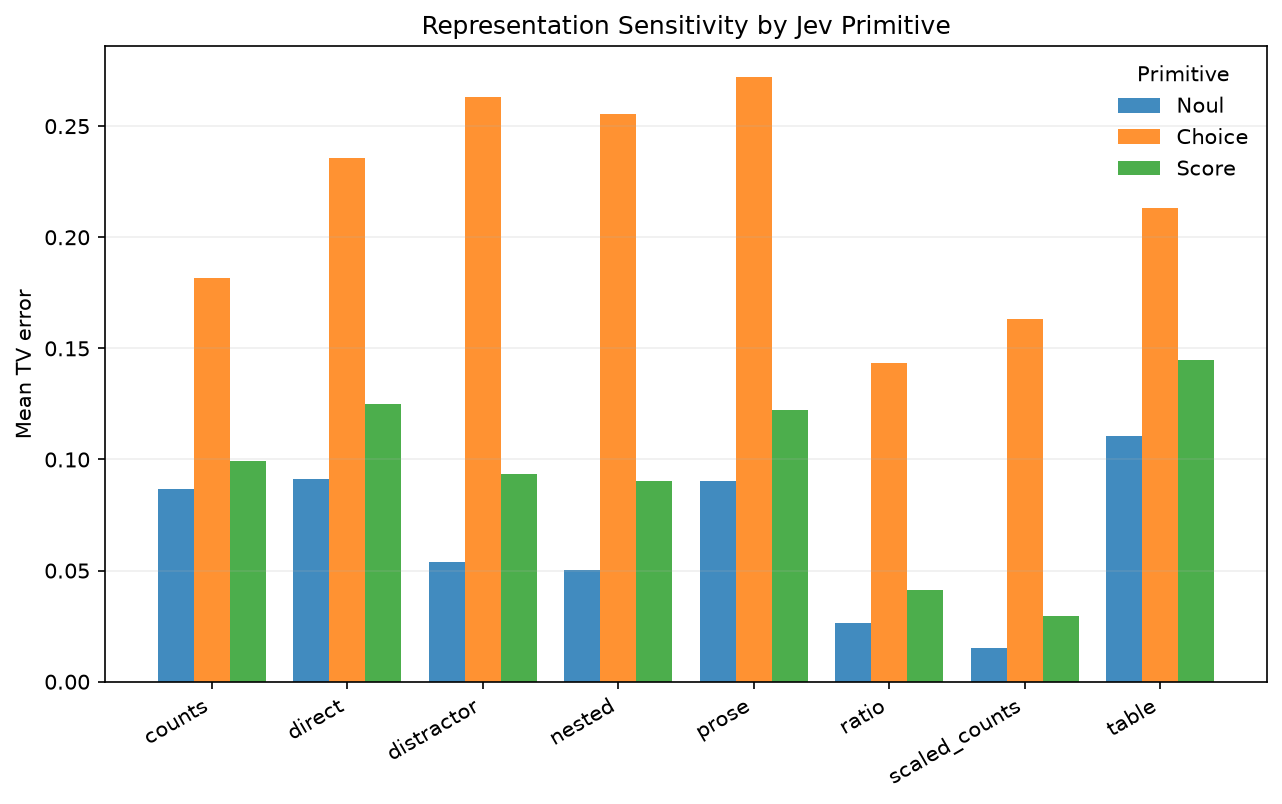
\includegraphics[width=0.7\columnwidth]{figure_3_representation_sensitivity.png}}
\caption{Representation sensitivity by primitive. \texttt{Choice} and SemIf are more sensitive to equivalent renderings than \texttt{Noul} or \texttt{Score} expectation.}
\label{fig:repr-sensitivity}
\end{figure}


\begin{table*}[t]
\caption{Examples of representation types in Sys1Cal-v1. Each row shows one rendered state format used to express an exact latent probability problem. The proposition and gold distribution are shared by the three primitives Noul, Choice, and Score.}
\label{tab:representation-examples}
\begin{center}
\scriptsize
\begin{tabular}{llp{0.4\textwidth}p{0.15\textwidth}}
\toprule
Representation & Family & State & Proposition / gold \\
\midrule
Direct &
Explicit probability &
\texttt{sufficient\_statistics:} $p_A=0,\;p_{\neg A}=1$ &
``Event A is true.'' \newline
$P(\mathrm{True})=0$ \\\\
\hline
Ratio &
Explicit probability &
\texttt{probability\_ratio\_A\_to\_not\_A: 0:1} &
``Event A is true.'' \newline
$P(\mathrm{True})=0$ \\\\
\hline
Prose &
Explicit probability &
Natural-language rendering: ``The state fully determines the target distribution. The probability of $A$ is 0, and the remaining probability belongs to the other outcome.'' &
``Event A is true.'' \newline
$P(\mathrm{True})=0$ \\
\hline
Distractor &
Explicit probability &
Same sufficient statistics as the direct form, plus irrelevant metadata &
``Event A is true.'' \newline
$P(\mathrm{True})=0$ \\\\
\hline
Counts &
Frequency &
\texttt{counts:} zor $=800$, nif $=200$; sampling is uniform over objects. &
``The sampled object is a zor.'' \newline
$P(\mathrm{True})=0.8$ \\\\
\hline
Scaled counts &
Frequency &
Equivalent count representation with all counts scaled: zor $=80000$, nif $=20000$. &
``The sampled object is a zor.'' \newline
$P(\mathrm{True})=0.8$ \\\\
\hline
Table &
Frequency &
A table with one row per label: zor has count 40, nif has count 10. &
``The sampled object is a zor.'' \newline
$P(\mathrm{True})=0.8$ \\\\
\hline
Nested state &
Conditional probability &
Nested contingency state with counts:
$A\wedge B=74$, $A\wedge \neg B=48$, $\neg A\wedge B=79$, $\neg A\wedge \neg B=55$;
query is $P(A\mid B)$. &
``Event A is true.'' \newline
$P(\mathrm{True})=0.484$ \\
\bottomrule
\end{tabular}
\end{center}
\end{table*}

\end{document}